\subsection{Les industriels responsables et la garantie longue durée}


L'obligation d'une garantie légale est souvent présentée comme une alternative face à \\l'\op. Il existe dans les faits déjà quelques propositions de marques connues ou non dans ce sens.

\bigbreak
Contrairement aux garanties légales, la garantie contractuelle ou commerciale peut être offerte ou non selon la décision du vendeur. Pour cette raison, elle est considérée facultative par rapport aux garanties légales. Le vendeur est obligé de respecter les dispositions qui régissent ces garanties légales, et d'en informer l'acheteur. 
En raison de la garantie commerciale, et en cas de panne, le professionnel prend en charge la réparation de l'appareil tant que la période de garantie n'est pas terminée. Il peut aussi proposer de remplacer le produit.

\bigbreak
Lorsque le fabricant accorde une garantie supplémentaire pour son produit, celle-ci est nommée « garantie constructeur » ou « garantie fabricant ». Cette garantie ne devient valide que si le vendeur ne propose pas une garantie commerciale \cite{loigarantie}.
On retrouve cet exemple avec la multinationale \textit{Apple} qui fournit une garantie fabricant d'un an \cite{apple}. Cet acte est tout à fait normal car toutes les entreprises du domaine électrique et électronique offrent le plus souvent des garanties d'un an. Mais ici, \textit{Apple} laisse croire à ses clients que la garantie du produit n'est valable qu'une seule année depuis la date d'achat du produit, et qu'ensuite, le produit n'est plus garanti. Ceci est tout à fait légal mais l'entreprise américaine joue sur la différence entre la garantie constructeur qui dure un an et les garanties légales qui durent deux ans et plus, et il joue sur l'ignorance de ses clients des garanties qui existent aujourd'hui.

\bigbreak
Aujourd'hui, on commence à voir des entreprises ou des commerçants qui offrent des garanties de longue durée pour leurs produits. C'est le cas de la société anglaise d'électroménager \textit{Dyson}\footnote{http://www.dyson.com}, qui a proposé des aspirateurs avec une garantie longue de cinq ans. Ce qui veut dire que \textit{Dyson} offre trois ans de garantie de plus \cite{dyson}. Normalement pour bénéficier d'une telle garantie, le client devrait payer le prix normal du produit plus une augmentation liée à la garantie,au contraire de la proposition de la marque \textit{Dyson}.

\bigbreak
Le secteur automobile, lui aussi a osé proposer des garanties de longue durée, par l'intermédiaire de la marque \textit{KIA}. Jusqu'à aujourd'hui, le constructeur automobile sud-coréen avec son modèle \textit{CEE'D}\footnote{http://www.kia.com/fr/fr/modeles/nouvelle-ceed}, reste le seul à proposer une garantie gratuite de sept ans ou 150 000 kilomètres \cite{kia}. Ceci est difficile pour les Européens qui conservent leur voiture pour presque sept ans. Malheureusement, pour les automobilistes, peu de marques ont suivi l’initiative de la marque \textit{KIA}. Ainsi, si le client veut vendre sa voiture pendant la durée de la garantie indiquée dans sept ans, c'est le nouvel acheteur qui profitera du reste de la garantie. Cependant, les constructeurs automobiles européens restent avec des garanties de deux ans.

\bigbreak
On trouve aussi, l'entreprise néerlandaise \textit{Philips} qui a décidé de prendre en compte les conséquences écologiques de l'obsolescence programmée, notamment les produits jetables. Ces dernières années, \textit{Philips} a dirigé son investissement vers  les produits durables. L'un de ces produits durables est l'ampoule \textit{LED}\footnote{http://www.philips.fr/c-m-li/ampoules-led} (Light Emitting Diode), en français la diode électrolumi\-nescente ou la diode qui  diffuse de la lumière , cette ampoule a une durée de vie de 25 ans à l'opposée de l'ampoule à incandescence qui dure 2 000 heures (presque 2 ans), elle consomme un peu plus de 3 watts d’électricité quand l'ampoule à incandescence utilise 25 watts d’électricité \cite{ampoule_inc}. 


\bigbreak
Contrairement à \textit{Apple}, le \textit{PhoneBloks}\footnote{https://www.phonebloks.com} est une des idées innovantes qui a pour but de lutter contre l'obsolescence programmée. C'est l'idée d'un designer néerlandais \textit{Dave Hakkens}\footnote{http://www.davehakkens.nl} qui cherchait à inventer une smartphone complètement personnalisable basé sur un système de briques comme présenté ci-dessous \cite{op_pb}.
\begin{figure}[h]
\begin{minipage}{0.5\linewidth}
\begin{center}
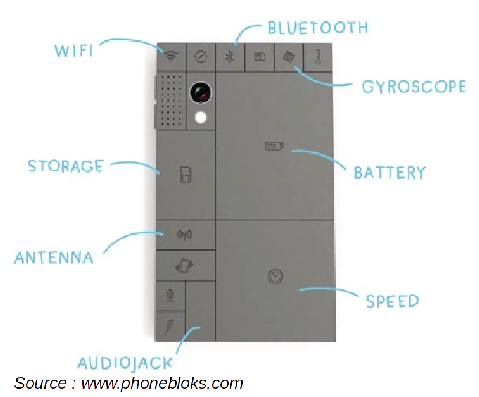
\includegraphics[scale=0.6]{Rsc/phonebloks2.png} 
\end{center}
\end{minipage}
\begin{minipage}{0.5\linewidth}
\begin{center}
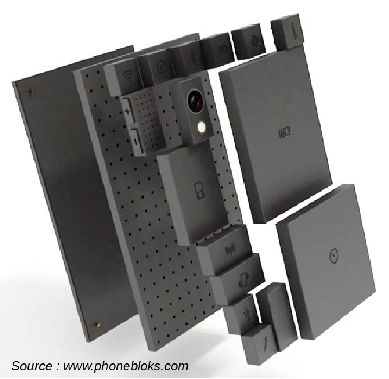
\includegraphics[scale=0.7]{Rsc/phonebloks1.png} 
\end{center}
\end{minipage}
\caption{\scriptsize{Phonebloks : le téléphone qui se monte et se démonte en quelques secondes.}}
\label{phonebloks}
\end{figure}

\bigbreak
Le principe ici, c'est que le téléphone mobile est un ensemble de composants aux différentes fonctions ( Wifi, batterie, GPS, Bluetooth, appareil photo, etc) et en cas de panne d'un composant, il suffit juste de le décrocher et le changer. 
Même si elle toujours dans la phase de conception, l'initiative a connu un grand succès sur les réseaux sociaux. La vidéo de la présentation du \textit{Phonebloks} sur \textit{Youtube} a déjà dépassé les 20 millions de vues \cite{pb_yt}, ce qui prouve qu'il y une vraie volonté des consommateurs qui ont soutenu le projet d'avoir un smartphone avec ses fonctionnalités très puissantes, un smartphone anti-obsolescence. Motorola a également présenté le Project Ara, qui reprend le concept de téléphone portable modulable.

\bigbreak
Quelques fabricants font donc l'effort d'offrir des produits de qualité, certes plus chers, mais surtout sous garantie. Cette initiative semble donc viable pour ces entreprises, et pourrait peut-être être appliquées par d'autres marques dans les années à suivre. Mais certains fabricants isolés ne font pas forcément pencher la balance, et c'est pourquoi quelques politiques ont essayé de faire adopter de nouvelles lois protégeant le consommateur.

%cite{loigarantie}

%cite{apple}

%cite{dyson}

%cite{kia}

%cite{ampoule_inc}

%cite{op_pb}

%cite{pb_yt}


